%Experimental Results and Analysis – in this section, you should show the quantitative results – charts and tables. Analyze the results by explaining and highlighting what is important on them in terms of your goals and what is bad. You should explain the strange results too.

%V ďalšej časti prezentujte vlastný prínos a vlastné výsledky porovnajte s výsledkami iných. Charakterizujte použité metódy.
%Vyhýbajte sa používaniu žargónu.
%Používajte starú múdrosť: 1 obrázok je viac než 1000 slov.

\subsection{4-2-4 Encoder} 
\label{sec:results-auto4} 

%TODO robustness 

%==================================================================
\paragraph{Introduction.} 
\label{sec:results-auto4-introduction} 
In this section, we analyse TLR~(\ref{sec:our-tlr}) performance for a broad range of parameters $\lambda_h$ and $\lambda_v$. The network architecture is only 4-2-4~
(\ref{sec:datasets-auto4}) what allows us to run plethora of simulations. There were two kinds of simulations. First were \emph{two dimensional maps (TDM)} where we plotted $\lambda_v$ on the $x$ axis, $\lambda_h$ on the $y$ axis and used color for the $z$ axis. Second were \emph{timelines} (TL) where a best configuration found by TDM was analysed. For TDM we ran about 200-500 networks for each ($\lambda_v$, $\lambda_h$) and for timelines about 5000-10000 runs. After the simulation ended we took the average for each parameter setting. The networks were trained while $patSucc^F \neq 0$ or $epoch < Epoch_{\rm max}$ where $Epoch_{\rm max}$ was set to 100,000 in TDM and 1,000,000 in TL. Note that most of the plots are in \emph{logarithmic} scale. 

%============================================================

\subsubsection{Comparison} 
\label{sec:tlr-auto4-cmp} 

In the following table~(\ref{tab:results-cmp-auto4}) we can see the comparison of the most important models which we analysed on the \emph{4-2-4 encoder} task. We achieved an improvement of BAL $patSucc^F$ from $62.7\%$ to $93.1\%$ by using two different learning rates~(\ref{sec:our-tlr}). This result was improved further to $99.86\%$ by preselecting networks based on initial weights~(\ref{sec:sim-exp-candidates}). This proved that hidden distance and representation convexity are important attributes of BAL~(\ref{sec:results-candidates}). 

On the other hand, many of the analysed models achieved poorly. Notably we tried modified GeneRec learning rules~(\ref{sec:models-generec-modifications}) on BAL, calling this model \emph{BAL GeneRec Learning Rules (BAL GLR)}. This led to no good results. Also, \emph{BAL-recirc}~(\ref{sec:our-bal-recirc}) achieved worse than BAL. We experimented with \emph{momentum} in section~(\ref{sec:results-momentum}), symmetric version of BAL in section~(\ref{sec:our-bal-sym}) and other modification but all without significant improvement in success. 

\begin{table}[H] 
  \centering
    \begin{tabular}{|l|l|l|l|l|}
    \hline
    Algorithm (section)&$\lambda_h$&$\lambda_v$&$patSucc^F$ &Epochs\\ %&SEM(success) \\
    \hline
    BP~(\ref{sec:models-bp}) &2.4 &2.4 &100&60\\ %&5.1\\
    \hline
    GR~(\ref{sec:models-generec}) &0.6 &0.6 &90&418\\ %&28\\
    \hline
    GR Sym~(\ref{eq:models-generec-learning-rule-sym}) &1.4 &1.4 &56&88\\ %&2.9\\
    \hline
    GR Mid~(\ref{eq:models-generec-learning-rule-mid}) &2.4 &2.4 &92&60\\ %&3.4\\
    \hline
    CHL~(\ref{sec:models-chl}) &1.2 &1.2 &56&77\\ %&1.8\\
    \hline
    BAL~(\ref{sec:models-bal})&0.9 &0.9 &62.7& 5136.11\\ %&2.0e+08\\
    \hline
    BAL TLR~(\ref{sec:our-tlr})&0.0002  & 500&93.12&5845.01\\ %&1.52e+08\\
    \hline
    BAL TLR Can~(\ref{sec:sim-exp-candidates})&0.0002&500&99.86&150.417\\ %&5,070,000\\
    \hline
    BAL Recirc~(\ref{sec:our-bal-recirc})&0.0001&1.0&36.0&1221.6\\ %&4.31e+07\\
    \hline
    BAL GLR~(\ref{sec:models-generec-modifications})& any & 0 & 0 & N/A \\ 
    \hline 
    %TODO Symmetric BAL 
    \end{tabular}
  \caption{Comparing performance of different models on the \emph{4-2-4 encoder} task. Data for BP, GR, GR Sym, Gr Mid and CHL are taken from~\citet{o1996bio}.} 
  \label{tab:results-cmp-auto4}
\end{table}

Note that when comparing runtime in table~\ref{tab:results-cmp-auto4} based on \emph{epochs} we must be aware of that GeneRec and BAL-recirc epochs take longer than others. That is because the recirculation step~(\ref{sec:models-generec-activation}) where usually about 5--15 iterations are necessary for activation to settle~(\ref{sec:generec-fluctuation}). Thus the 418 epochs of GeneRec are comparable to the 5845 epochs of TLR in terms of compuration time. 
 

%============================================================
\subsubsection{Two learning rates} 
\label{sec:tlr-auto4}

On figure~\ref{fig:results-tlr-auto4-performance} we compare success rate for different settings of $\lambda_v$ and $\lambda_h$. It~is interesting that the subspace with best achieving networks is around the half line $(10, 0.001)$ to $(10^9, 0.001)$. That means the result mainly depends on $\lambda_h$. Even more interesting is the epochs needed for successful networks where an \emph{rift} occurred around line $(0.01, 0.0002)$ to $(10^9, 0.0002)$. Unfortunatelly, we can only guess what is the reason behind this rift. Maybe it~is related to $Epoch_{\rm max}$ and the fact that we are calculating only for successful networks and therefore, networks having $\lambda_h < 10^{-6}$ converge fast because of $\lambda_v$ or fail to converge because of very small $\lambda_h$. 

%======== (3D) L1 x L2 x epochs =========
%======== (3D) L1 x L2 x patSuccF =========
\begin{figure}[H]
  \centering
  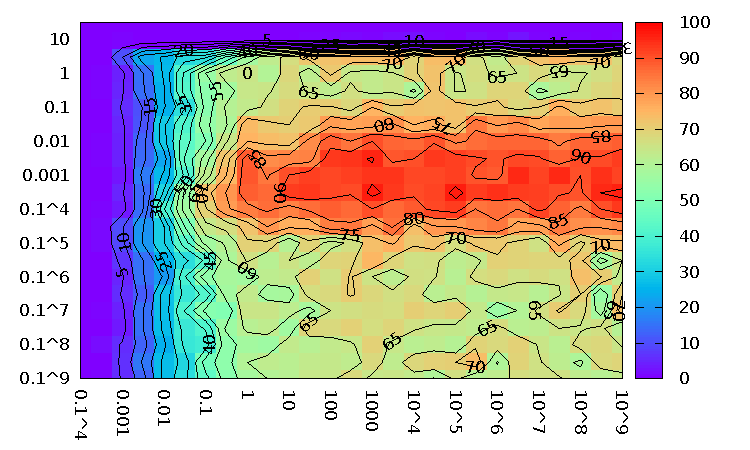
\includegraphics[width=0.49\textwidth]{img/tlr-auto4-success.pdf}   
  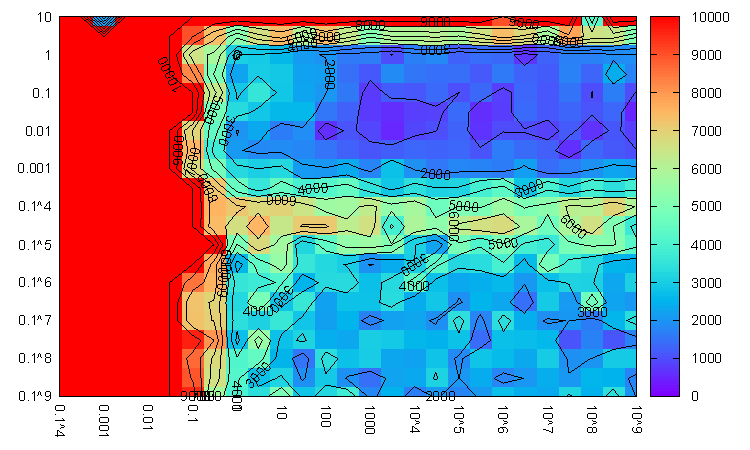
\includegraphics[width=0.49\textwidth]{img/tlr-auto4-epoch.pdf}     
  \caption{TLR success and epochs needed for successful networks on the \emph{4-2-4 encoder} task with $\sigma = 2.3$ and $\mu = 0.0$ best being $96.5\$$ with $\lambda_h=0.0003$ and $\lambda_v=1000.0$.}
  \label{fig:results-tlr-auto4-performance}
\end{figure}

Note the inconsistency between table~\ref{tab:results-cmp-auto4} where 93.12\% success was stated for TLR and in figure~\ref{fig:results-tlr-auto4-performance} it was 96.5\%. We can explain this by the \emph{law of big numbers}. In the first case we run 10,000 networks and therefore, the result is likely to mirror the reality. In the second case only 200 networks were run for each$(\lambda_v,\,\lambda_h)$ pairs with having about 50 candidates for best achievers. Thus if we do little amount of runs for these 50 candidates it~is likely that some them will achieve better than in reality. 

On figure~\ref{fig:results-tlr-auto4-epoch} the success timeline for TLR with best $\lambda_h$ and $\lambda_v$ is analysed. We see that the success rate increases even after $10^5$ epochs and our intuition tells us that it will continue even after $10^6$ epoch. Also interesting is that $patSucc^B$ first follows $patSucc^F$ for about 100 epochs but then it stagnates at rate $\approx0.8$ and even it starts to drop a little. %TODO explain, maybe an implementation error? It~is so symmetric and weight update is independent on activation cimputation. 

%======== (2D) best TLR on ALL_SUCC x epoch (std-dev) ==========
\begin{figure}[H]
  \centering
  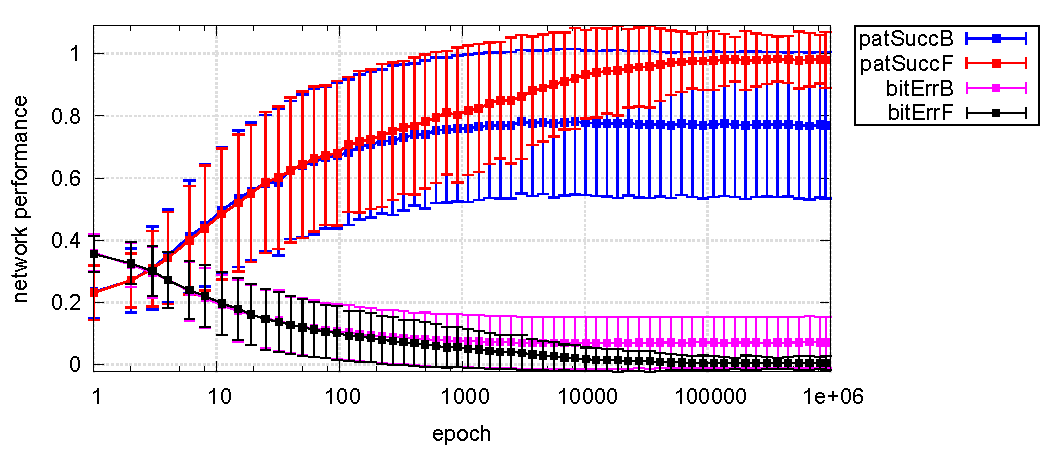
\includegraphics[width=0.8\textwidth]{img/tlr-auto4-best-perf.pdf}\\
  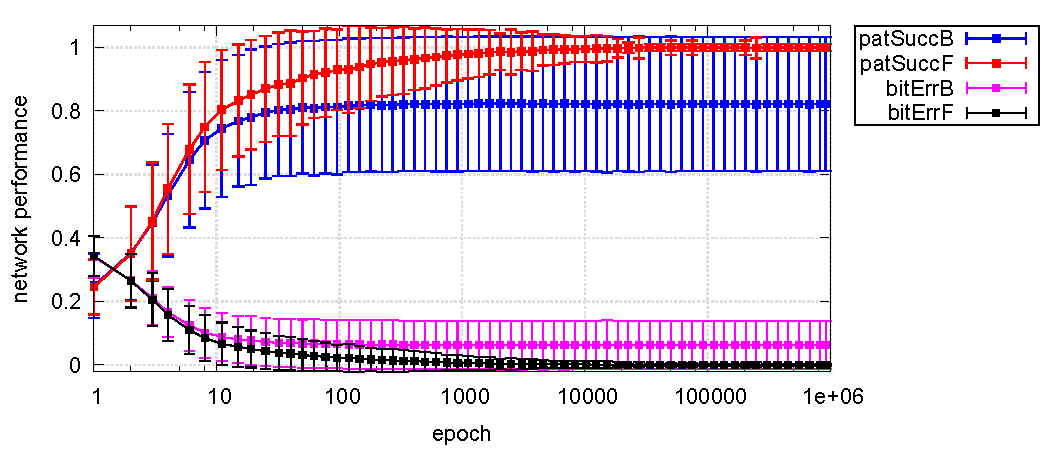
\includegraphics[width=0.8\textwidth]{img/tlr-auto4-best-can.pdf}      
  \caption{TLR success timeline for the \emph{4-2-4 encoder} task with $\lambda_h=0.0002$ and $\lambda_v=500$. Top without candidate selection and bottom with candidates selection.}
  \label{fig:results-tlr-auto4-epoch} 
\end{figure}

%============================================================
\subsubsection{Hidden activations} 
\label{sec:tlr-auto4-hidden}

On figures~\ref{fig:results-hidden-activations-bal} and~\ref{fig:results-hidden-activations-tlr} we show forward hidden activations. Each color represents the forward hidden representation of one of the four inputs in the \emph{4-2-4 encoder} task. As the hidden layer has size 2 it could be mapped to $(0,1)^2$. The activations started at the black dots and continued as outlined by the the lines. The numbers attached to the lines are the epoch numbers. 

The main difference between TLR and BAL seems to be the speed of activation change. In BAL on figure~\ref{fig:results-hidden-activations-bal} we have a step of size 0.6 which corresponds to four, one for each input, weight updates. And after some initial steps BAL tends to stop the activation change. This could be contributed to settling $|H^F-H^B| \approx 0$ as discussed in~(\ref{sec:our-hidden-activation}). 

Another source of error could be \emph{non--convex} hidden activation initializations. In the beginning the weight matrices are initialized by random what leads to random hidden activations. If they are also non--convex in the end then it~is impossible to perfectly classify on the hidden--to--visible layer due the linear separability theorem discussed in section~(\ref{sec:models-perceptron}). Thus the network must \emph{escape} the non convex state which could introduce problems. 

%TODO empty page 

%===== hidden activation timelines with commentaries (for TLR, BAL, GeneRec) 
% 2x success, 2x error (wrong settle, divergence) 

\begin{figure}[H]
  \centering
  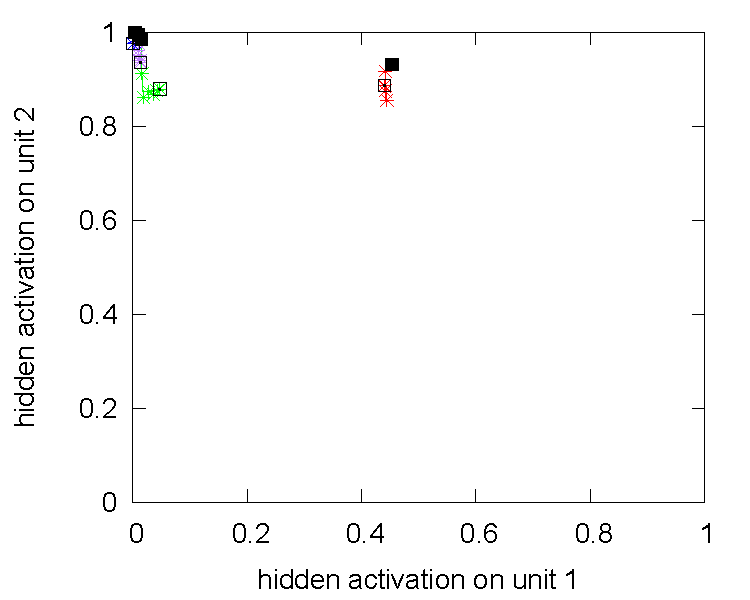
\includegraphics[width=0.45\textwidth]{img/hid-bal-bad-init.pdf}  
  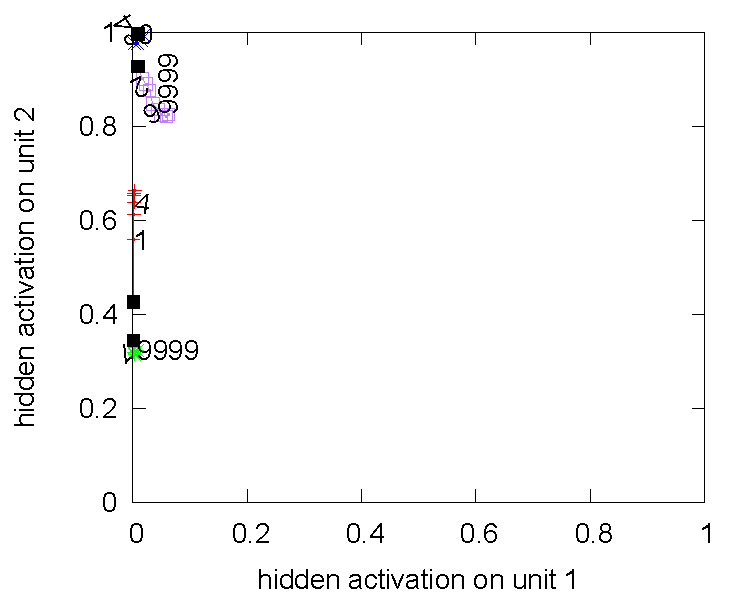
\includegraphics[width=0.45\textwidth]{img/hid-bal-bad-convex.pdf}  \\
  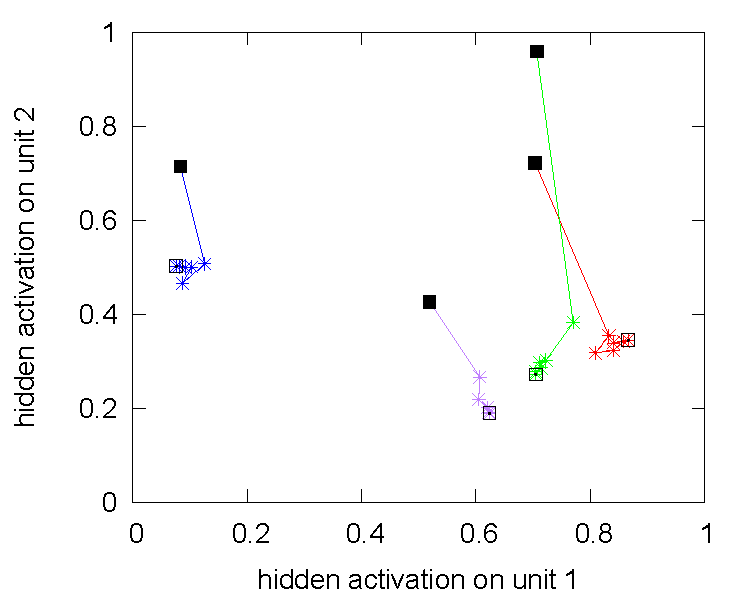
\includegraphics[width=0.45\textwidth]{img/hid-bal-bad-step.pdf}  
  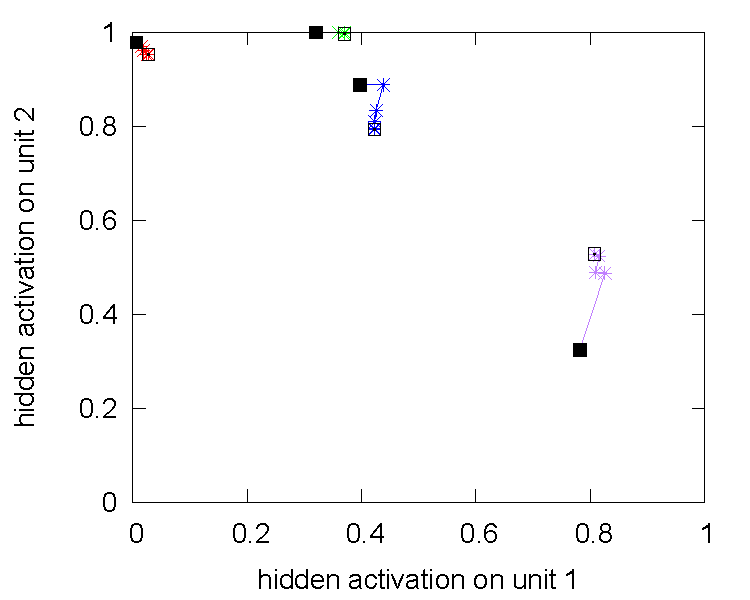
\includegraphics[width=0.45\textwidth]{img/hid-bal-bad-stagnation.pdf}  \\
  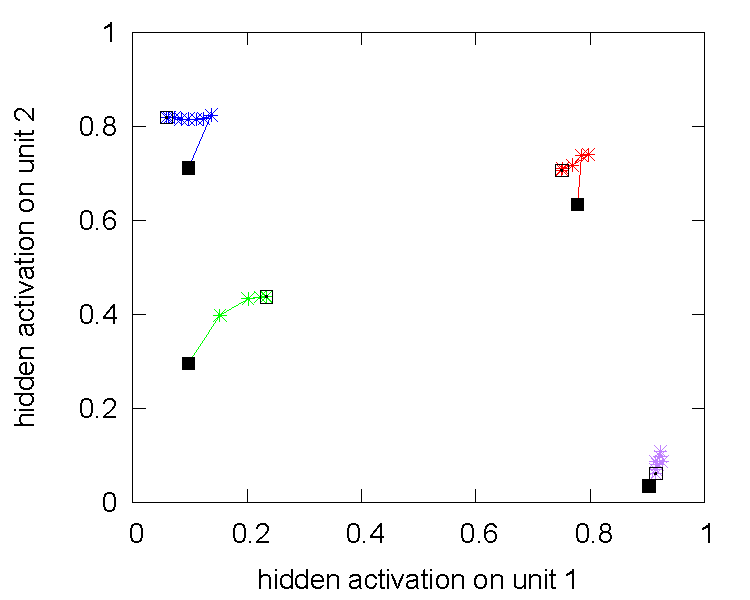
\includegraphics[width=0.45\textwidth]{img/hid-bal-good-init.pdf}  
  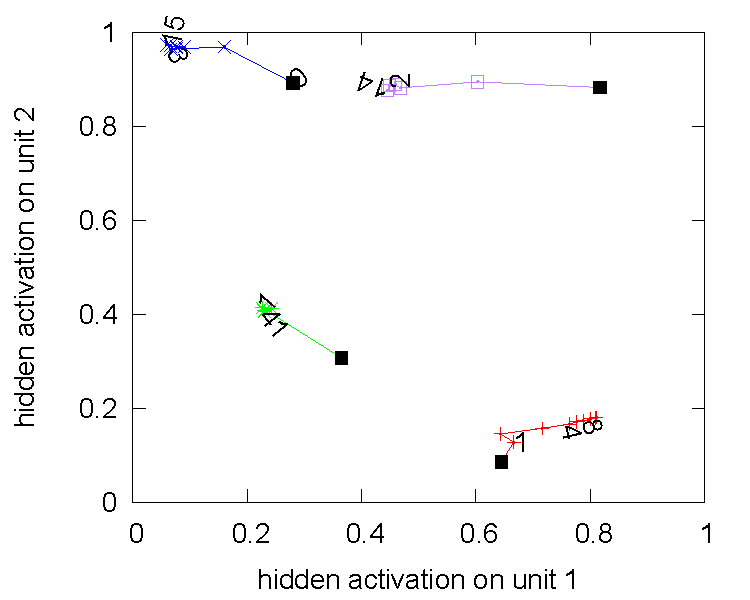
\includegraphics[width=0.45\textwidth]{img/hid-bal-good-convex.pdf}  \\
  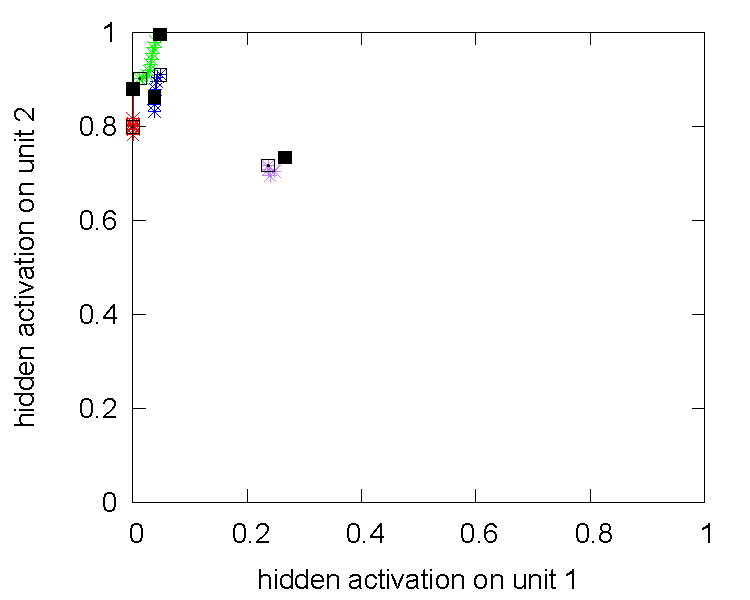
\includegraphics[width=0.45\textwidth]{img/hid-bal-good-step.pdf}  
  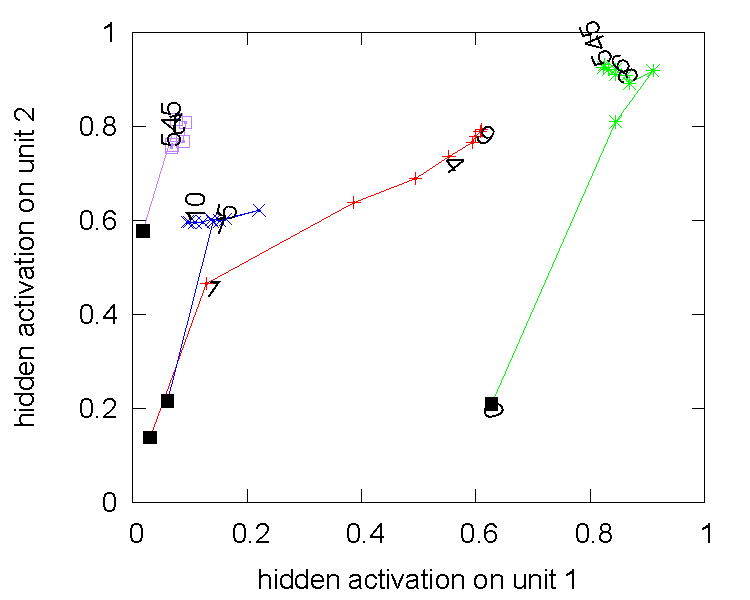
\includegraphics[width=0.45\textwidth]{img/hid-bal-good-stagnation.pdf}  \\ 
  \caption{\emph{BAL} hidden activations on the \emph{4-2-4 encoder}. Top $2\times2$ are {\bf un}successful networks and bottom $2\times2$ successful ones. Filled square depicts the start and empty space the end.}
  \label{fig:results-hidden-activations-bal}
\end{figure}

\begin{figure}[H]
  \centering
  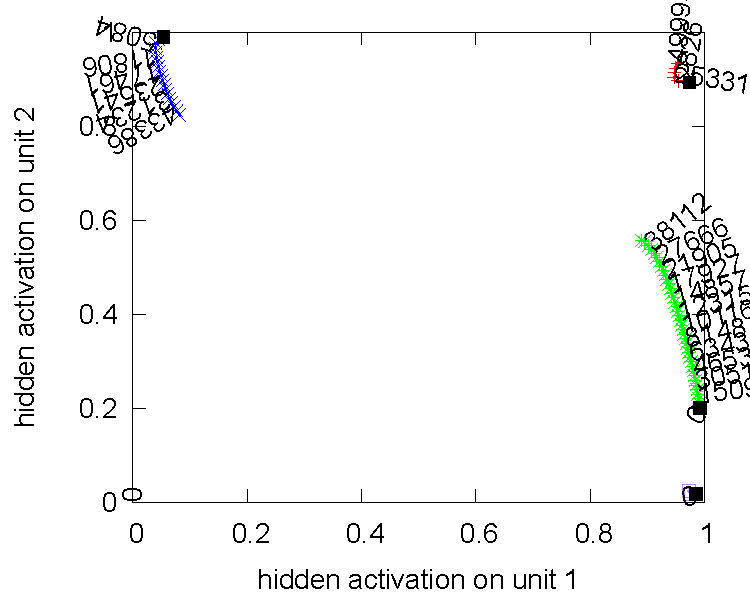
\includegraphics[width=0.45\textwidth]{img/hid-tlr-bad-static.pdf}  
  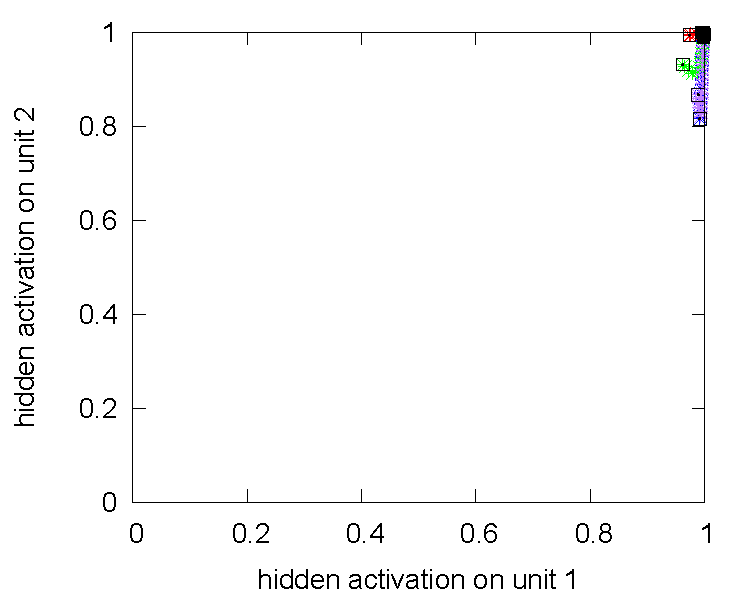
\includegraphics[width=0.45\textwidth]{img/hid-tlr-bad-tiny.pdf}  
  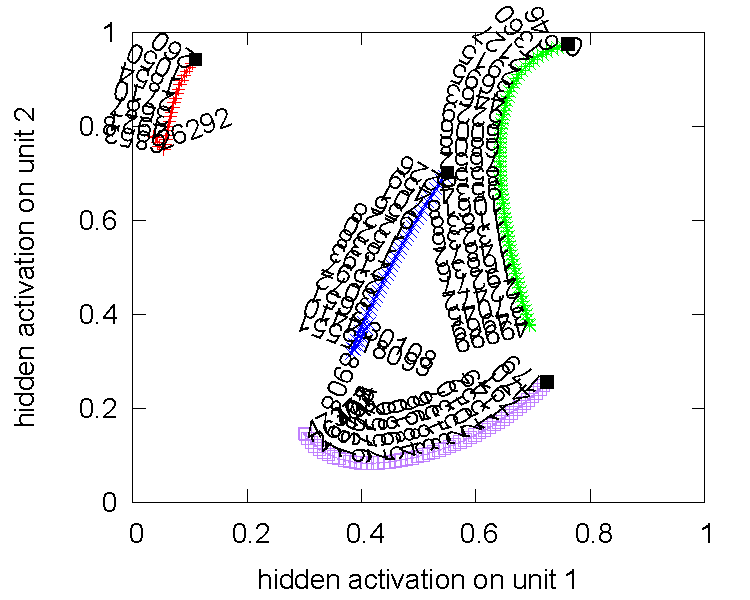
\includegraphics[width=0.45\textwidth]{img/hid-tlr-bad-init.pdf}  
  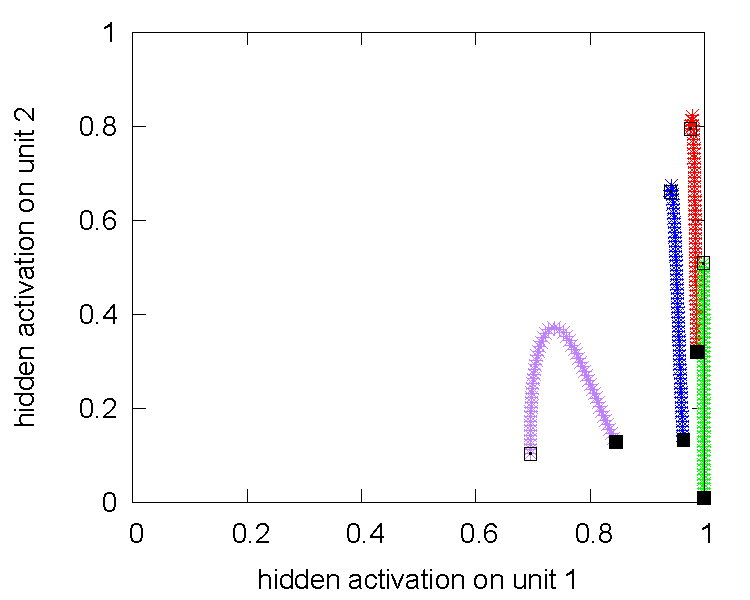
\includegraphics[width=0.45\textwidth]{img/hid-tlr-bad-weird.pdf}  
  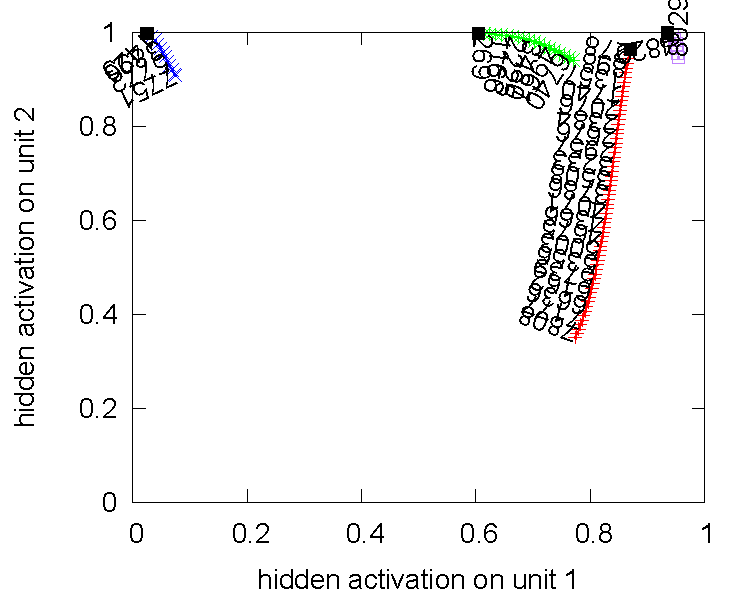
\includegraphics[width=0.45\textwidth]{img/hid-tlr-good-static.pdf}  
  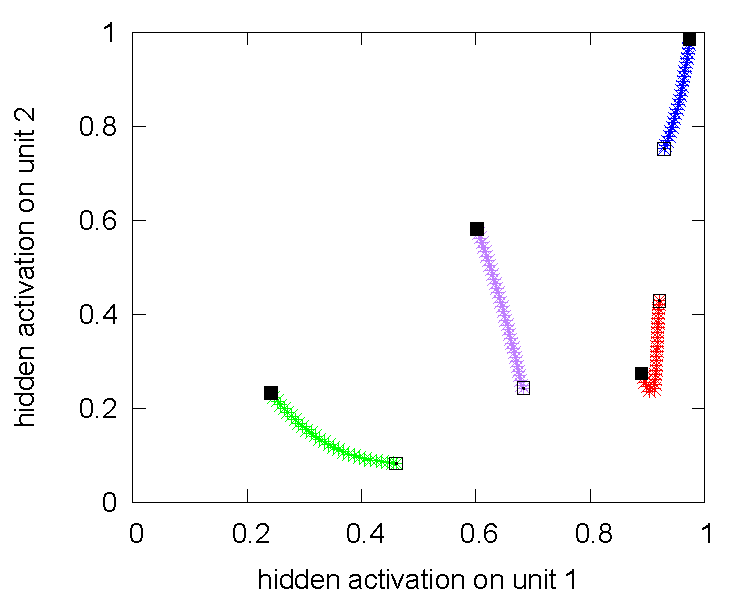
\includegraphics[width=0.45\textwidth]{img/hid-tlr-good-tiny.pdf}  
  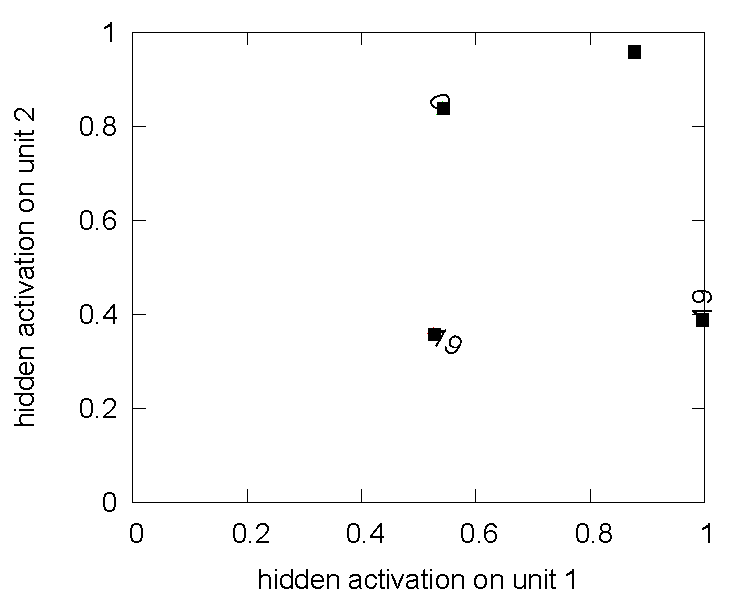
\includegraphics[width=0.45\textwidth]{img/hid-tlr-good-init.pdf}  
  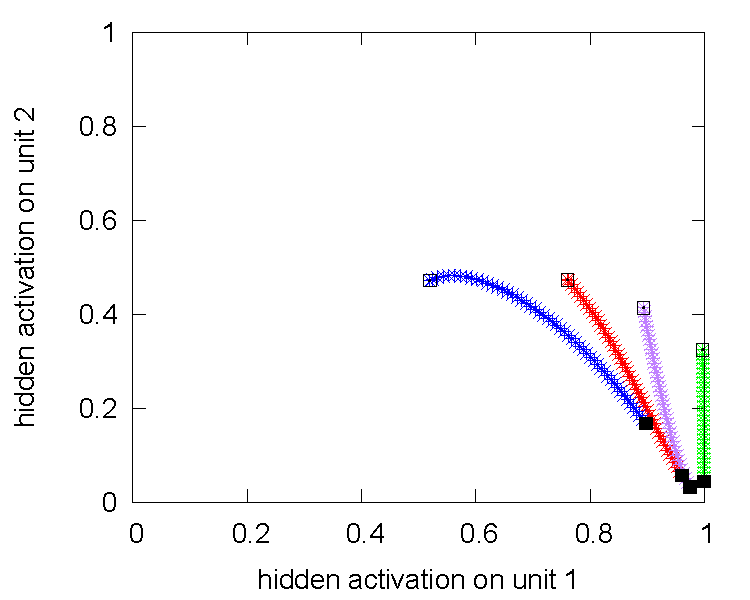
\includegraphics[width=0.45\textwidth]{img/hid-tlr-good-weird.pdf}  
  \caption{\emph{TLR} hidden activations on the \emph{4-2-4 encoder}. Top $2\times2$ are {\bf un}successful networks and bottom $2\times2$ successful ones. Filled square depicts the start and empty space the end.}
  \label{fig:results-hidden-activations-tlr}
\end{figure}

%========================================================
\subsubsection{Momentum}
\label{sec:results-momentum} 

Momentum (\ref{sec:our-momentum}) had no significant effect on network performance as shown in table~\ref{tab:results-mom-auto4}. Only a little improvement in convergence rate was achieved. The simulations were ran accross multiple $\lambda_v$ and $\lambda_h$ corresponding to figure~\ref{fig:results-tlr-auto4-momentum}. Then the average from all simulations was taken. 
\begin{table}[H] 
  \centering
  {\small
    \begin{tabular}{|l|l|}
    \hline
momentum & avg(success) \\
    \hline
0.001  & 0.4419 \\
    \hline
0.003  & 0.4428 \\
    \hline
0.01   & 0.4440 \\
    \hline
0.03   & 0.4464 \\
    \hline
0.1    & 0.4468 \\
    \hline
0.3    & 0.4493 \\
    \hline
    \end{tabular}
  }
  \caption{Comparing performance of different models on the \emph{4-2-4 encoder} task.} 
  \label{tab:results-mom-auto4}
\end{table}

%======== (3D) L1 x L2 x patSuccF : TLR vs. best momentum =========
%======== (3D) L1 x L2 x epochs : TLR vs. best momentum =========

\begin{figure}[H]
  \centering
  \includegraphics[width=0.49\textwidth]{img/tlr-mom-auto4-success-0-001.pdf}  
  \includegraphics[width=0.49\textwidth]{img/tlr-mom-auto4-epoch-0-001.pdf}  \\
  \includegraphics[width=0.49\textwidth]{img/tlr-mom-auto4-success-0-3.pdf}  
  \includegraphics[width=0.49\textwidth]{img/tlr-mom-auto4-epoch-0-3.pdf}  
   \caption{Comparing momentums $\mu=0.01$ (top) and $\mu=0.3$ (bottom) for TLR on the \emph{4-2-4 encoder} task.}
  \label{fig:results-tlr-auto4-momentum}
\end{figure}


%============================================================
\subsubsection{Features}
TODO explain 

\begin{figure}[H]
  \centering
  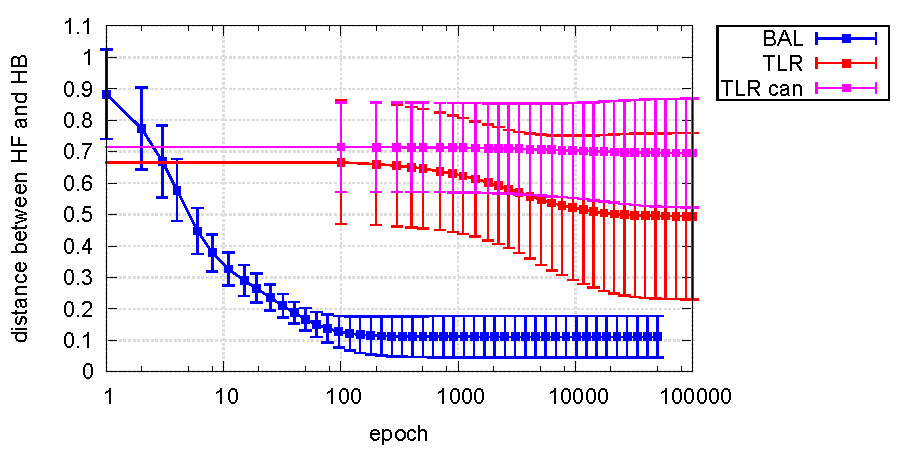
\includegraphics[width=0.6\textwidth]{img/feature-cmp-h-fb-d.pdf}  
   \caption{Comparing $dist_{H}^{FB}$~(\ref{sec:our-dist-h-fb}) evolution on the {4-2-4 encoder} task.}
  \label{fig:results-candidates-h-fb-d}
\end{figure}

\begin{figure}[H]
  \centering
  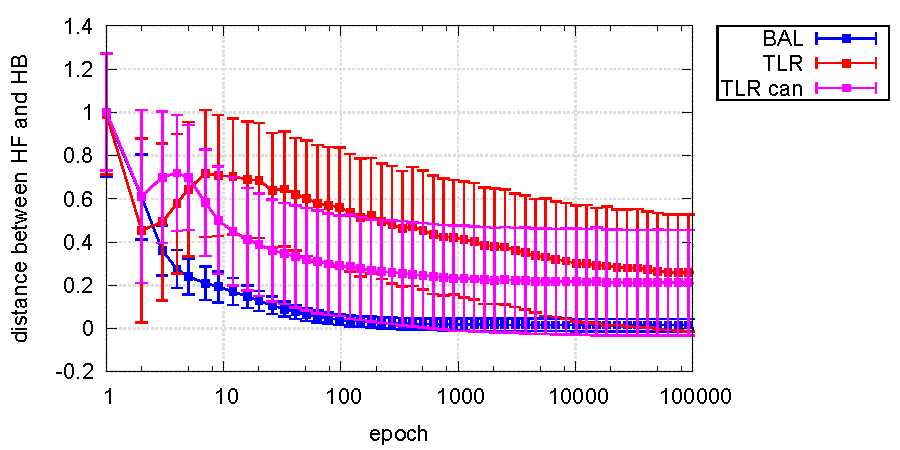
\includegraphics[width=0.6\textwidth]{img/feature-cmp-o-fb-d.pdf}  
   \caption{Comparing $dist_{O}^{FB}$~(\ref{sec:our-dist-o-fb}) evolution on the {4-2-4 encoder} task.}
  \label{fig:results-candidates-o-fb-d}
\end{figure}

\begin{figure}[H]
  \centering
  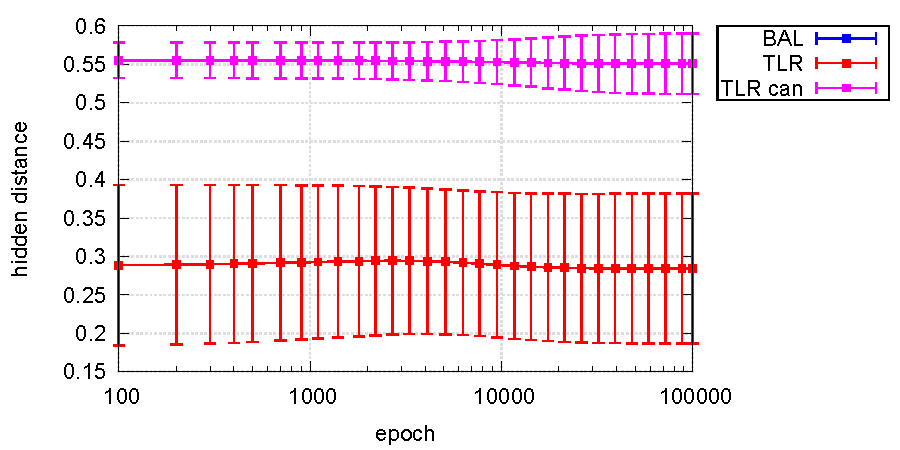
\includegraphics[width=0.6\textwidth]{img/feature-cmp-h-dist.pdf}  
   \caption{Comparing $dist_{H}$~(\ref{sec:our-h-dist}) evolution on the {4-2-4 encoder} task.}
  \label{fig:results-candidates-h-dist}
\end{figure}

\begin{figure}[H]
  \centering
  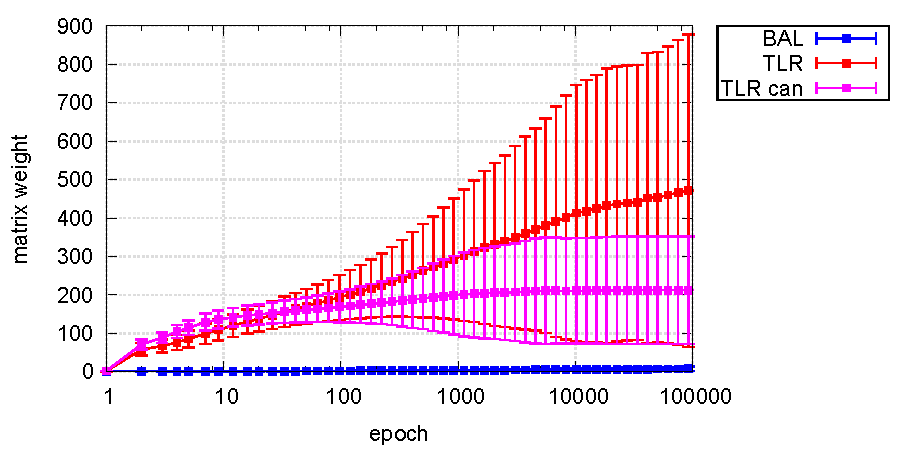
\includegraphics[width=0.6\textwidth]{img/feature-cmp-m-wei.pdf}  
   \caption{Comparing $matrix\_weight$~(\ref{sec:our-m-wei}) evolution on the {4-2-4 encoder} task.}
  \label{fig:results-candidates-m-wei}
\end{figure}


\subsubsection{Other}

\paragraph{Recirculation BAL.} 
On figure~\ref{fig:results-bal-recirc-auto4-performance} we see that \emph{BAL-recirc}~(\ref{sec:our-bal-recirc}) achieved lower success rate than BAL on the \emph{4-2-4 encoder} task. In comparison with TLR we see that there is a global maxima at point $\lambda_h = 0.0001$ and $\lambda_v=1.0$. We can therefore conclude that the space of possible improvement by parameters $\lambda_h$ and $\lambda_v$ is bounded. Similar results were achieved for GeneRec as shown on figure~\ref{fig:results-generec-auto4-performance}.
%======== (3D) L1 x L2 x epochs =========
%======== (3D) L1 x L2 x patSuccF =========
\begin{figure}[H]
  \centering
  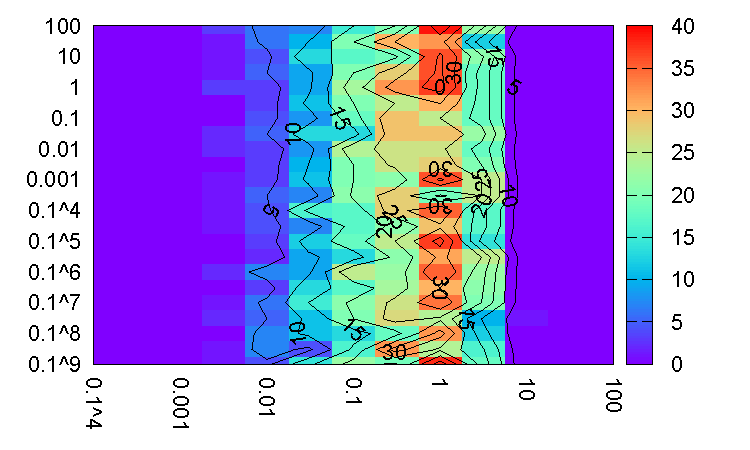
\includegraphics[width=0.49\textwidth]{img/bal-recirc-auto4-success.pdf}   
  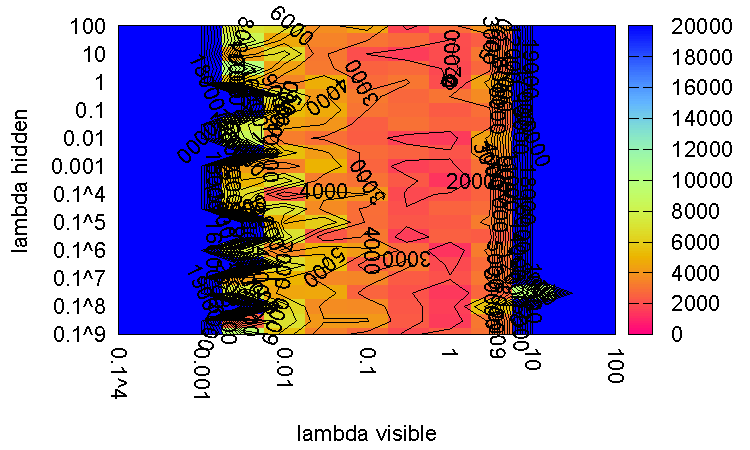
\includegraphics[width=0.49\textwidth]{img/bal-recirc-auto4-epoch.pdf}     
  \caption{BAL-recirc~(\ref{sec:our-bal-recirc}) success and epochs on the \emph{4-2-4 encoder}. Best result $36\%$ achieved with $\lambda_h = 0.0001$ and $\lambda_v=1.0$.}
  \label{fig:results-bal-recirc-auto4-performance}
\end{figure}
%success lambda_h lambda_v
%33.0 0.0003 1.0
%33.0 0.001 3.0
%34.0 0.01 1.0
%36.0 0.0001 1.0
%36.0 3.0e-05 0.3


\paragraph{GeneRec.} 
As with generalizing of BAL to TLR we tried also generalizing GeneRec with the two learning rates approach. The results shown on figure~\ref{fig:results-generec-auto4-performance} shows no increase in success rate in comparison with setting $\lambda_v = \lambda_h$, i.e. original GeneRec. It is also similar with the result of BAL-recirc show on figure~\ref{fig:results-bal-recirc-auto4-performance} that the success space is bounded.  
%======== (3D) L1 x L2 x epochs =========the
%======== (3D) L1 x L2 x patSuccF =========
\begin{figure}[H]
  \centering
  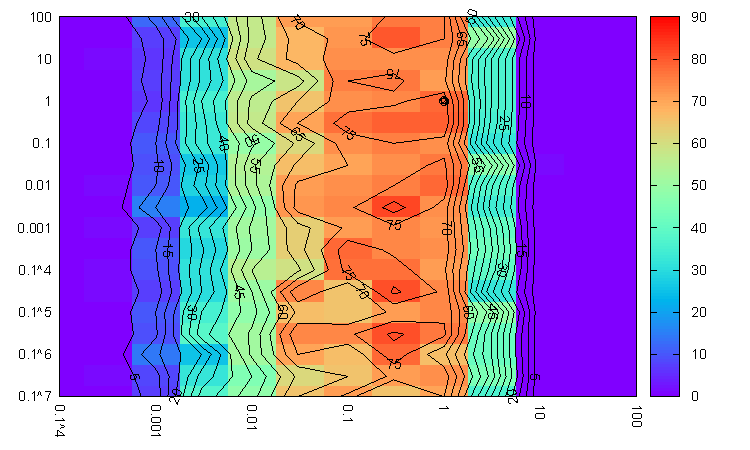
\includegraphics[width=0.49\textwidth]{img/generec-auto4-success.pdf}   
  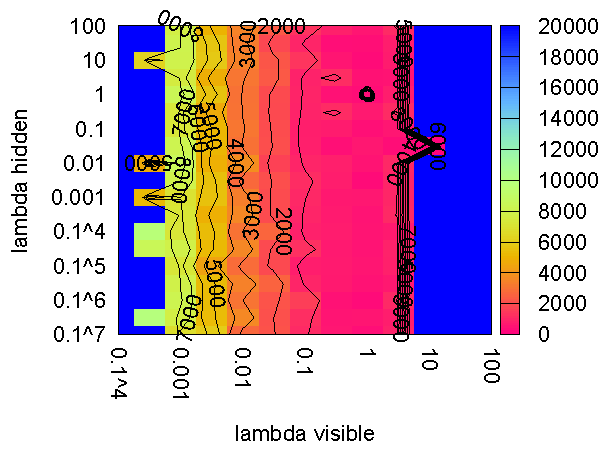
\includegraphics[width=0.49\textwidth]{img/generec-auto4-epoch.pdf}     
  \caption{GeneRec~(\ref{sec:models-generec}) success and epochs on the \emph{4-2-4 encoder} task with $\sigma = 2.3$ and $\mu = 0.0$. Best result $83\%$ achieved with $\lambda_h = 0.3$ and $\lambda_v=1.0$.}
  \label{fig:results-generec-auto4-performance}
\end{figure}

%77.0 1.0 0.1
%78.0 1.0 0.3
%81.0 0.3 0.3
%83.0 0.3 1.0

%TODO[opt] 
%\paragraph{Symmetric BAL.} 
%\label{sec:our-bal-sym} 
%We were inspired by the necessary condition for convergence of GeneRec as stated by~\citet{o1996bio}. Thus we introduced \emph{Symmetric BAL (SymBAL)} as a modification of BAL where we set symmetric weights $W^{IH} = (W^{HI})^T$ and $W^{HO} = (W^{OH})^T$. We found no significant improvement when using this approach. TODO plot. 

\subsubsection{Conclusion} 
\label{sec:tlr-auto4-conclusion} 

\label{sec:tlr-auto4-hypothesis} 
We could introduce a hypothesis why TLR outperforms BAL on the \emph{4-2-4 encoder task}. The hypothesis is suggested by sections on hidden distances~(\ref{sec:tlr-auto4-hidden}) and~(\ref{sec:our-hidden-activation}) and on candidate selection~(\ref{fig:results-tlr-auto4-epoch}). The reason is that the hidden activations settle to fast. This is explained by the fact that forward and backward hidden activations become same to fast and moreove, the weight initialization could help this. These issues are solved by $\lambda_h \ll \lambda_h$ which adds epochs to the training phase and by candidate selection which prevents initializing hidden activations close to each other. 

